\documentclass[12pt]{article}
\usepackage[utf8]{inputenc}
\usepackage[margin=3cm]{geometry}
\usepackage{float}
\usepackage{graphicx}
\usepackage{physics}
\usepackage{amsmath}
\usepackage{amssymb}
\usepackage[colorlinks]{hyperref}
\usepackage{subcaption}
%\captionsetup{font=footnotesize}
\usepackage{booktabs}
\usepackage{multirow}
\usepackage{newtxtext, newtxmath}
\newcommand{\otoprule}{\midrule[\heavyrulewidth]}
\usepackage[export]{adjustbox}
\usepackage{cite}

\title{DS Instability in an Annular (Corbino) Geometry}
\author{Jack Farrell}
\begin{document}
	\maketitle
	\section{Equations}
	We study the equations:
	\begin{equation}
	\label{eq:mainEquation}
	\begin{aligned}[c]
	\pdv{J}{t} + \pdv{r}\left(\frac{J^2}{n} + n \right) -\frac{\eta}{m} \left(\pdv[2]{r} + \frac{1}{r}\pdv{r}\right)\frac{J}{n} = \gamma (J_0 - J) - \frac{J^2}{n} \frac{1}{r},  \\
	\pdv{n}{t} + \pdv{J}{r} = -\frac{J}{r}. \\
	\end{aligned}
	\end{equation}
	\section{Asymmetric Boundary Conditions}
	Consider first the generalization of the ``asymmetric" boundary conditions from ~\cite{Mendl2019}:
	\begin{equation}
	\begin{aligned}
	\left.\pdv{r}(rJ)\right|_{r=R_1}&=0, \\
	J(r=R_2)&=v_0, \\
	n(r=R_1)&=1. \\
	\end{aligned}
	\end{equation}
	
	\subsection{Quasinormal Modes}
	We linearize Eqs. (\ref{eq:mainEquation}) with respect to the small perturbations $J=J_0 + J_1e^{-\mathrm{i}\omega t}$, $n = n_0+n_1e^{-\mathrm{i}\omega t}$.  The resulting, a Bessel Equation, can be solved numerically.  At $v_0 = 0.14$, $\eta=0.01$, and $\gamma = 0.04$, Fig. (\ref{fig:symmetricFrequencies}) shows the dependence of these values on the ratio $\mathcal{R}\equiv L/R_1$.  In the limit of small $\mathcal{R}$, you get:
	
	\begin{equation}
	\label{eq:analyticFreq}
	\omega \approx \left(\frac{\pi}{2}  -\frac{\mathcal{R}}{\pi}\right) + \mathrm{i}\left(v_0(1+2\mathcal{R}) - \frac{\gamma}{2} - \frac{\eta \pi^2 n^2}{8}\right)
	\end{equation}
	
	\begin{figure}[ht]
		\centering
		\includegraphics[width=\textwidth]{../../Figures/annular-frequency-growthrate.pdf}
		\caption{Frequency and Growth Rate of the quasinormal modes under asymmetric boundary conditions.  The solid black line gives the value for $\mathcal{R}=0$, which corresponds to the rectangular geometry.}\label{fig:symmetricFrequencies}
	\end{figure}

	Increasing $\mathcal{R}$, making the problem ``more annular" decreases the oscillation frequency.  But at the same time, the growth rate becomes larger.  That means the instability should persist at lower $v_0$ or higher $\eta$ and $\gamma$, each of which could be desirable experimentally.
	
	\subsection{Simulations}
	Let's try first changing the ratio $\mathcal{R}$ and keeping the other parameters ($v_0$, $\eta$, $\gamma$) constant.  Those results are given in Fig. (\ref{fig:vary-ratio}).
	
	\begin{figure}[ht]
		\centering
		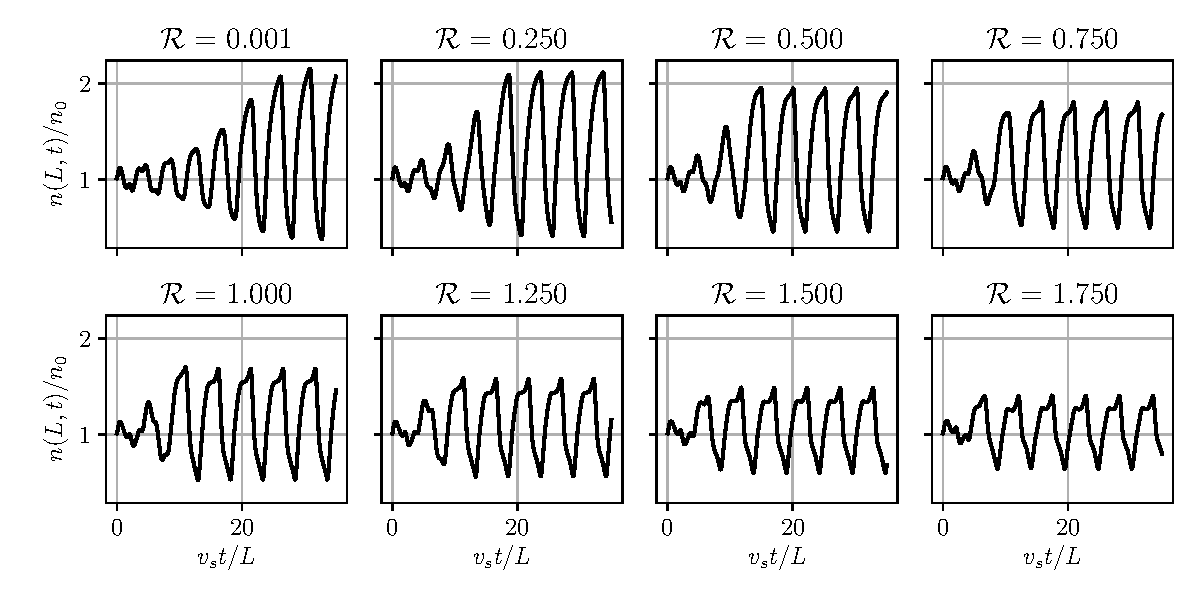
\includegraphics[width=\textwidth]{../../../Corbino/Figures/vary-ratio/vary-ratio.pdf}
		\caption{Keeping other parameters constant, change the ratio $\mathcal{R}$.}\label{fig:vary-ratio}
	\end{figure}
	
	As expected, we notice a decrease in the oscillation frequency as $\mathcal{R}$ increases.  The instability also grows faster at higher $\mathcal{R}$.  But the amplitude of the endpoint of the instability decreases with greater $\mathcal{R}$.  I think this is a nonlinear effect--- the linearized solutions would say the frequency keeps growing. 
	
	Let's check if we do find an instability in an area of parameter-space where we wouldn't have in the rectangular geometry.  Eq.(2) of ~\cite{Mendl2019} suggests that there should be \textit{no} instability at the parameters $v_0 = 0.04$, $\eta=0.01$, $\gamma=0.1$.  But running the simulation does give an instability as long as $\mathcal{R}$ is large enough.  For instance, for $\mathcal{R}=2.500$, the results are shown in Fig. (\ref{fig:check-existence}).
	
	\begin{figure}[ht]
		\centering
		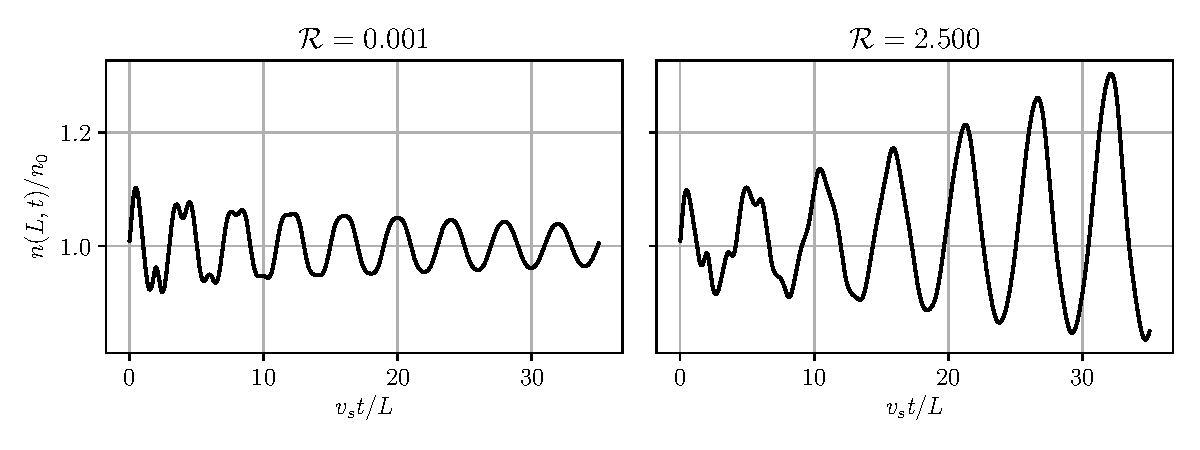
\includegraphics[width=\textwidth]{../../../Corbino/Figures/check-existence/check-existence.pdf}
		\caption{When $\mathcal{R}=0.001$, which basically corresponds to the rectangular geometry, there is no instability.  But the instability reappears at, for instance, $\mathcal{R}=2.500$.}\label{fig:check-existence}
	\end{figure}
	
	\section{Symmetric Boundary Conditions}
	In the rectangular geometry, it's the asymmetric boundary conditions that allow the instability.  But a paper I found from 2010, ~\cite{Sydoruk2010}, guessed that since the annulus has a geometric asymmetry between the electrodes already, one might be able to get away with symmetric boundary conditions.  By considering linearized equations, they found that the instability should exist and has \textit{double the frequency} of the rectangular case.  But they don't have any viscosity or relaxation.  The boundary conditions are:
	\begin{equation}
	\label{eq:symmetricBC}
	n(r = R_1) = n(r = R_2) = 0.
	\end{equation}
	I'll note that through the continuity equation, this puts a Neumann-like condition on the momentum $J$ as well. 
	
	\subsection{Quasinormal Modes}
	Anyway, I solved the linearized equations numerically with these new boundary conditions, and I found that we do get a higher frequency and an instability that is favoured at higher $\mathcal{R}$, as summarized in Fig. (\ref{fig:symmetricBCfreq}).
	
	\begin{figure}[ht]
		\centering
		\includegraphics[width=\textwidth]{../../Figures/frequency-growthrate-symmetric.pdf}
		\caption{Using the symmetric boundary conditions (\ref{eq:symmetricBC}).}\label{fig:symmetricBCfreq}
	\end{figure}
	The parts with negative imaginary $\omega$ have no instability--- but, with increasing $\mathcal{R}$, it quickly goes positive.  So the instability should exist--- but I haven't been able to observe the endpoint numerically yet.  I suspect I'm overconstraining it, because I'm trying right now to apply four boundary conditions: two Dirichlet conditions on the density, and two Neumann-like conditions on the momentum.  The best I can do right now is plot it in a regime where the instability is not supposed to exist, and at least show that the frequency is higher.  That's given in Fig. (\ref{fig:symmetric-boundary}).
	
	\begin{figure}[ht]
		\centering
		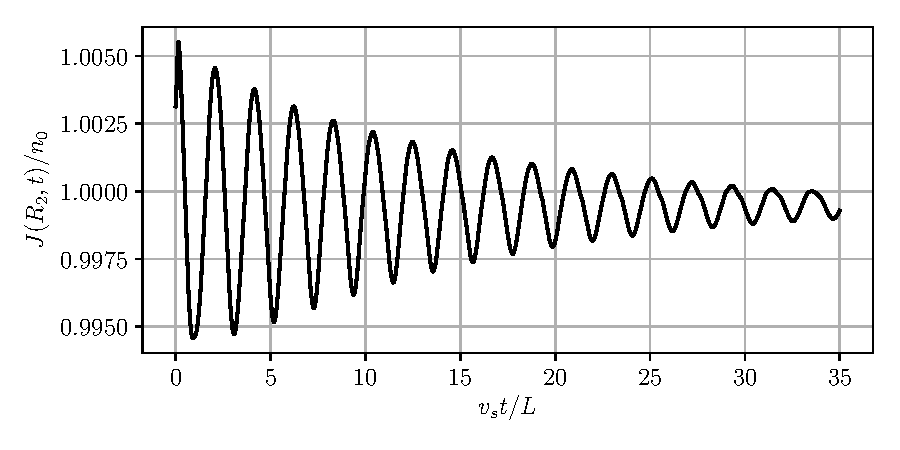
\includegraphics[]{../../../Corbino/Figures/symmetric-boundary/symmetric-boundary.pdf}
		\caption{Solution with symmetric boundary conditions.  While the oscillations have double the frequency, so far, I have only seen decay.}\label{fig:symmetric-boundary}
	\end{figure}
	
	\bibliography{../../../Corbino/References/DSInstability}{}
	\bibliographystyle{plain}
\end{document}